\documentclass[a4paper,11pt,twoside]{memoir}

\setcounter{secnumdepth}{2} % Niveau de profondeur pour la numérotation

\let\STARTCODE\relax 
\let\STOPCODE\relax 
\STARTCODE
\usepackage{color,calc,graphicx,soul}
\definecolor{nicered}{rgb}{.647,.129,.149} \makeatletter
\newlength\dlf@normtxtw \setlength\dlf@normtxtw{\textwidth}
\def\myhelvetfont{\def\sfdefault{mdput}} \newsavebox{\feline@chapter}
\newcommand\feline@chapter@marker[1][4cm]{%
  \sbox\feline@chapter{%
    \resizebox{!}{#1}{\fboxsep=1pt%
      \colorbox{nicered}{\color{white}\bfseries\sffamily\thechapter}%
    }}%
  \rotatebox{90}{%
    \resizebox{%
      \heightof{\usebox{\feline@chapter}}+\depthof{\usebox{\feline@chapter}}}%
    {!}{\scshape\so\@chapapp}}\quad%
  \raisebox{\depthof{\usebox{\feline@chapter}}}{\usebox{\feline@chapter}}%
} \newcommand\feline@chm[1][4cm]{%
  \sbox\feline@chapter{\feline@chapter@marker[#1]}%
  \makebox[0pt][l]{% aka \rlap
    \makebox[1cm][r]{\usebox\feline@chapter}%
  }} \makechapterstyle{daleif1}{
%   \setlength{\beforechapskip}{0pt}
%   \setlength{\midchapskip}{0pt}
  \setlength{\afterchapskip}{10pt}
%   \setlength{\chapindent}{0pt}
  \renewcommand{\insertchapterspace}{}
  \renewcommand\chapnamefont{\normalfont\Large\scshape\raggedleft\so}
  \renewcommand\chaptitlefont{\normalfont\huge\bfseries\scshape\color{nicered}}
  \renewcommand\chapternamenum{} 
  \renewcommand\printchaptername{}
%  \renewcommand\printchapternum{\vspace{-5.5cm}\null\hfill\feline@chm[2.5cm]\par}
  \renewcommand\printchapternum{\vspace{-1.8cm}\null\hfill\feline@chm[2.5cm]\par}
  \renewcommand\afterchapternum{\par\vskip\midchapskip}
  \renewcommand\printchaptertitle[1]{\chaptitlefont\raggedleft
    ##1\par}
%  \renewcommand\printchapternonum{\vspace{-3.5cm}}
  \renewcommand\printchapternonum{\vspace{0.2cm}}
 %  \renewcommand{\insertchapterspace}{}
}

\makeatother
\chapterstyle{daleif1}
\STOPCODE

%%% Fin du modèle de rapport de stage
%%%%%%%%%%%%%%%%%%%%%%%%%%%%%%%%%%%%%%%%%%%%%%%%%%%%%%%%%%%%%%%


\usepackage[a4paper]{geometry} %% CG : à desactiver avec la classe "orsay-thesis"
\geometry{left=3cm,right=3cm,top=2.5cm} % proposition, CG: à désactiver si classe "orsay-thesis" utilisée

\usepackage[utf8]{inputenc}
\usepackage[T1]{fontenc}
\usepackage[english, french]{babel} % Pour une thèse en français et en anglais
% puis dans le corps du document utiliser...
%\selectlanguage{frenchb} % pour écrire en français
%\selectlanguage{english} % pour écrire en anglais


\usepackage{lipsum} %Pour faire des essais

% Choix de la langue
%\usepackage[greek,english,frenchb]{babel}


% Lmodern et substitution des petites capitales grasses manquantes
\usepackage{lmodern}
\rmfamily
\DeclareFontShape{T1}{lmr}{b}{sc}{<->ssub*cmr/bx/sc}{}
\DeclareFontShape{T1}{lmr}{bx}{sc}{<->ssub*cmr/bx/sc}{}


%%%%%%%%%%%%%%%%%%%%%%%%%%%%%%%%%%%%%%%%%%%%%%%%%%%%%%%
% Modifications Cyril Grouin (nouveaux packages, corrections, adaptations)
%%%%%%%%%%%%%%%%%%%%%%%%%%%%%%%%%%%%%%%%%%%%%%%%%%%%%%%

%% --- Mise en page globale : épigraphe ; lettrine ; mini tables des
%% matières ; numéro des pages des appels de référence dans la
%% bibliographie ; exemples numérotés ; boîtes ovales colorées autour
%% du texte ; séparateur "feuille de vigne"
\usepackage{epigraph}
%\usepackage{lettrine} %% CG: erreurs à la compilation mais fonctionne
\usepackage[french]{minitoc}
\setcounter{minitocdepth}{2} %% CG: Profondeur des niveaux
\usepackage{soul}
\usepackage[pagebackref,colorlinks=true,citecolor=forestgreen,linkcolor=black,menucolor=alezan,urlcolor=prune]{hyperref}
\renewcommand*{\backref}[1]{}
\renewcommand*{\backrefalt}[4]{%
\ifcase #1 %
-- Non cité.%
\or
-- Cité page~#2.%
\else
-- Cité pages~#2.%
\fi}
\renewcommand*{\backrefsep}{, }
\renewcommand*{\backreftwosep}{ et~}
\renewcommand*{\backreflastsep}{ et~}
\usepackage{lingmacros} % CG: exemples numérotés
\usepackage{fancybox} % CG: boîtes ovales dans le texte
\usepackage{pifont} % CG: pour intégrer des caractères spéciaux
\usepackage{dsfont} % CG: pour intégrer des caractères mathématiques
\def\sep{\begin{center}\begin{large}\ding{167}\end{large}\end{center}}

%% --- Noms de sections prédéfinies (bibliographie, liste des figures)
\renewcommand{\bibname}{Bibliographie}
\addto{\captionsenglish}{\renewcommand{\bibname}{Bibliographie}}
\addto{\captionsfrench}{\renewcommand{\listfigurename}{Liste des figures}}

%% --- Mise en forme locale : polices de caractères ; couleurs ;
%% tableaux (fusion de lignes, rotation des labels, tableaux sur
%% plusieurs pages, barre oblique dans une cellule) ; intégration de
%% code informatique ; suppression des espaces devant la ponctuation ;
%% police de caractères Matrix Script Bold en version Regular
%\renewcommand{\rmdefault}{lcm} % Déclaration globale
\usepackage{newcent} % bookman, chancery, charter, newcent, palatino, times, utopia
\usepackage{helvet} % avant, helvet
\usepackage{color}
\usepackage{colortbl}
\usepackage{multirow}
%\usepackage{adjustbox}
\usepackage{longtable}
%\usepackage{slashbox}
\newcommand{\withnofdp}[1]{{\NoAutoSpaceBeforeFDP #1}}
\usepackage{arydshln} %% lignes pointillés dans les tableaux

\usepackage{listings}
\lstset{
  language=XML, 
  basicstyle=\small, % the size of the fonts that are used for the code, footnotesize
  showspaces=false, % show spaces adding particular underscores
  showstringspaces=false, % underline spaces within strings
  breaklines=true, % sets automatic line breaking
  breakatwhitespace=true, % sets if automatic breaks should only happen at whitespace
  morecomment=[s]{<!--}{-->},
  alsoletter=.-,
  commentstyle=\itshape\color{gray},
  markfirstintag=true,
  string=[d]",
  keywords={correction},
  keywordstyle=\color{alizarine},
  stringstyle=\color{acier},
}

%% --- Graphismes (Tikz, PGF) : courbes, histogrammes, cartes
%% mentales, arbres de dépendances ; définitions de codes couleur
%% personnels
\usepackage{pgf,pgfarrows,pgfnodes}
\usepackage{tikz}
\usepackage{tikz-qtree} % CG: pour les arbres
\usepackage{tikz-dependency} % CG: pour les dépendances
\usepackage{pgfplots}
\usetikzlibrary{mindmap,trees, backgrounds}
\usepackage{filecontents}
\usepackage{qtree}
\definecolor{acier}{HTML}{3A8EBA}
\definecolor{alezan}{HTML}{A76726}
\definecolor{alizarine}{HTML}{D90115}
\definecolor{amande}{HTML}{82C46C}
\definecolor{ambre}{HTML}{F0C300}
\definecolor{abricot}{HTML}{E67E30}
\definecolor{grey}{rgb}{0.9,0.9,0.9}
\definecolor{gris}{rgb}{0.1,0.1,0.1}
\definecolor{forestgreen}{rgb}{0.13,0.54,0.13}
\definecolor{dockerblue}{rgb}{0.11,0.56,0.98}
\definecolor{orange}{rgb}{0.64,0.16,0.16}
\definecolor{ocre}{HTML}{DFAF2C}
\definecolor{prune}{HTML}{811453}

%% --- Nouvelles commandes spécifiques à ce manuscrit
\newcommand{\remCyril}[1]{\textcolor{dockerblue}{\emph{CG : #1}}}%\color{black}}
\newcommand{\myex}[1]{\color{acier}{\emph{#1}}\color{black}}
\newcommand{\rg}[1]{\textsl{Remarque : #1}}
\def\euro{\mbox{\raisebox{.25ex}{{\it =}}\hspace{-.5em}{\sf C}}}

%%%%%%%%%%%%%%%%%%%%%%%%%%%%%%%%%%%%%%%%%%%%%%%%%%%%%%%


%% http://www.developpez.net/forums/d597791/autres-langages/autres-langages/latex/modifier-marge-page-ponctuellement/
%%%% debut macro %%%%
\newenvironment{changemargin}[2]{\begin{list}{}{%
\setlength{\topsep}{0pt}%
\setlength{\leftmargin}{0pt}%
\setlength{\rightmargin}{0pt}%
\setlength{\listparindent}{\parindent}%
\setlength{\itemindent}{\parindent}%
\setlength{\parsep}{0pt plus 1pt}%
\addtolength{\leftmargin}{#1}%
\addtolength{\rightmargin}{#2}%
}\item }{\end{list}}
%%%% fin macro %%%%

\usepackage{chngpage}
%\usepackage{chronology} % Package pourri, ne fonctionne pas avec Babel.
%\usepackage{timeline}
%\usepackage{chronosys} % Superpose les événements trop proches
%\usepackage{ulem} % remplace emph par du souligné


% Interligne
%\renewcommand{\baselinestretch}{1}


% Différents paquets pour les maths
\usepackage{amssymb,amsmath,amsthm,amscd}
\usepackage{mathrsfs}

% Pour les figures
\usepackage{subfig}

%Pour la page de garde
\usepackage{tabularx} % Permet d'utiliser l'environnement tabularx
\usepackage{calc} % Pour pouvoir donner des formules dans les définitions de longueur
\usepackage{graphicx} % Pour inclure des graphiques 
% Attention : pour inclure des .jpg comme dans l'exemple (ou des .png ou .pdf)
% il faut compiler directement en pdf (commande pdflatex).
% Pour inclure des .eps, il faut compiler avec latex + dvips + ps2pdf.

% Pour avoir des liens hypertexte dans le document compilé
\usepackage{hyperref}
%\usepackage{nohyperref} % à utiliser pour pouvoir compiler sans générer des liens

% Pour mettre la bibliographie dans la table des matières avec le bon numéro de page (voir plus loin)
%\usepackage[nottoc]{tocbibind}

% Pour l'index des notations
\usepackage{makeidx}
\makeindex

% Pour la nomenclature
\usepackage[french,intoc,refpage]{nomencl}
\renewcommand{\nomname}{Glossaire}
\renewcommand*{\pagedeclaration}[1]{\unskip\dotfill\hyperpage{#1}}
\makenomenclature


%% Essai pour supprimer l'entrée "Table des matières" de la table des matières
\newcommand{\nocontentsline}[3]{}
\newcommand{\tocless}[2]{\bgroup\let\addcontentsline=\nocontentsline#1{#2}\egroup}




% =========================== Commandes diverses ===============================

% Macros-commandes : appel à des fichiers extérieurs
%%%%%%%%%%%%%%%%%%%%%%%%%%%%%%%%%%%%%%%%%%%%%%%%%%%%%%%
%% EN-TETES ET PIEDS DE PAGE
\let\footruleskip\undefined
\usepackage{fancyhdr}
\pagestyle{fancy}% pour activer le style de pages personnalisé
\fancyhf{}%remise à zéro des en-tête et pied de page
\setlength{\headheight}{14pt} % pour fixer la hauteur de l'espace réservé à l'en-tête du haut

%%% Pas de numéro de page sur la première page des chapitres
\makeatletter
\let\ps@plain=\ps@empty
\makeatother

%===================== Style 1 =================================================
%En-tête : 
% * dans la boite de droite (R), pour les pages impaires (O)
% * et dans la boite de gauche (L), pour les pages paires (E)
% mettre le numéro de page (\thepage).
\fancyhead[RO,LE]{% 
\thepage
}
\fancyhead[LO]{\scshape \nouppercase{\rightmark}}  %%%Section
\fancyhead[RE]{\scshape \nouppercase{\leftmark}} %%% Chapitre 
\renewcommand{\headrulewidth}{.4pt}
\fancyfoot{}


%================================== Style 2 ====================================

% \fancyfoot[RO,LE]{% Boite de droite (R), pages impaires(O) et Boites de gauche pages paires
% \thepage
% }
% \fancyhead[CO]{\slshape \nouppercase{\rightmark}}  %%%Section
% \fancyhead[CE]{\slshape \nouppercase{\leftmark}} %%% Chapitre 
% \renewcommand{\headrulewidth}{.4pt}

% Remarques generales :
% nouppercase permet l'affichage en minuscules au lieu de majuscules
% slshape permet l'affichage en lettres penchés
% scshape permet l'affichage en petites capitales

% Pour que les pages paires sans texte (par exemple, à la fin d'un chapitre et
% avant un autre), ne contiennent ni en-tête ni pied de page (source :
% http://www.tex.ac.uk/cgi-bin/texfaq2html?label=reallyblank)
\let\origdoublepage\cleardoublepage
\newcommand{\clearemptydoublepage}{%
  \clearpage
  {\pagestyle{empty}\origdoublepage}%
}
\let\cleardoublepage\clearemptydoublepage

% Réglage fin des notes de bas de page
\FrenchFootnotes % pour les notes de bas de page à la française
\AddThinSpaceBeforeFootnotes % pour avoir une espace fine entre le mot et l'appel de note


%%%%%%%%%%%%%%%%%%%%%%%%%%%%%%%%%%%%%%%%%%%%%%%%%%%%%%%
%% CHAPITRE ETOILE
%% avec référence dans la table des matières et les bons en-têtes
%% il sert pour l'introduction, la page de notations.
\newcommand*\chapterstar[1]{%
  \chapter*{#1}%
  \addcontentsline{toc}{chapter}{#1}%
  \markboth{#1}{#1}}


%%%%%%%%%%%%%%%%%%%%%%%%%%%%%%%%%%%%%%%%%%%%%%%%%%%%%%%
% ENVIRONNEMENTS DE THEOREMES
\theoremstyle{plain} % style plain
\newtheorem{theo}{Théorème}[chapter]
\newtheorem{cor}[theo]{Corollaire}
\newtheorem{prop}[theo]{Proposition}
\newtheorem{lem}[theo]{Lemme}
\newtheorem{conj}[theo]{Conjecture}
\newtheorem*{theoetoile}{Théorème} % théorème non numéroté
\newtheorem*{conjetoile}{Conjecture} % conjecture non numérotée

\theoremstyle{definition} % style definition
\newtheorem{defi}[theo]{Définition}
\newtheorem{exemple}[theo]{Exemple}
\newtheorem{question}[theo]{Question}
\newtheorem{remarque}[theo]{Remarque}
\newtheorem{notation}[theo]{Notation}

% Pour renommer ``preuve'' en ``démonstration''
\renewcommand{\proofname}{Démonstration}


%%%%%%%%%%%%%%%%%%%%%%%%%%%%%%%%%%%%%%%%%%%%%%%%%%%%%%%
% ENVIRONNEMENTS DEDICACE ET EPIGRAPHE
\newenvironment{dedicace}{%
  \newpage\thispagestyle{empty}
  \hfill\begin{minipage}{100mm}\begin{flushright}\it}{%
  \end{flushright}\end{minipage}\vfill}

\newenvironment{epigraphe}{%
  \hfill\begin{minipage}{60mm}\begin{flushright}\footnotesize\it}{%
  \end{flushright}\end{minipage}\hspace*{7mm}\vfill}
 % macros diverses personnelles 
% (en-têtes et pieds de page, environnements de théorèmes) - voir macros.tex
%\input{macrosmath} % macros mathématiques - voir le fichier macrosmath.tex

% =========================== Commandes et paquets personnels ===============================
%\usepackage{moreverb} % utilisation de verbatimtab
%\usepackage{verbatim} % inclure du code source
\newcommand\tab[1][5mm]{\hspace*{#1}} % Insérer des tabulations.
\parindent=0em % Supprimer les marges en début de paragraphes.
%\usepackage{lilypond}

% =========================== Info du document =================================

% \title{Titre du m\'emoire}
% \author{Pr\'enom NOM}


% ================================ Debut du document ===========================

\begin{document}
\sloppy
\dominitoc

%%%%%%%%%%%%%%%%%%%%%%%%%%%%%%%%%%%%%%%%%%%%%%%%%%%%%%%%%%%%%%%%
%% Page de garde
%%%%%%%%%%%%%%%%%%%%%%%%%%%%%%%%%%%%%%%%%%%%%%%%%%%%%%%%%%%%%%%%
% ================================ Page du garde ==============================

\pdfbookmark[0]{Page de garde}{garde}
\thispagestyle{empty}

\begin{center}
  \begin{tabularx}{\textwidth}{m{10.3cm}m{4cm}}
	 
\includegraphics[width = 3.9cm]{images/logos/logo-inalco.png} %% CG : 3.5cm au lieu de 3 cm
	&
        %% TODO: remplacer le logo du LIMSI par celui de la société ou
        %% du laboratoire où vous avez réalisé votre stage (si le
        %% sujet du mémoire de recherche fait suite à votre stage)
	 
\includegraphics[width = 3.9cm]{images/logos/logo-inria.png} %% CG : 3.5cm au lieu de 3 cm
        \\ \hline
  \end{tabularx}
\end{center}

\begin{center}
\vspace{\stretch{1}}
% Permet de créer un espace vertical de longueur variable (\stretch) et de "poids" 1
{\Large \textbf{Institut National des Langues et Civilisations Orientales}}

\vspace{\stretch{1}}

{\normalsize Département Textes, Informatique, Multilinguisme}

\vspace{\stretch{2}}
\hrule
\vspace{\stretch{1}}
%% TODO: indiquez le titre de votre mémoire
{\LARGE \textbf{Titre du mémoire}}
\vspace{\stretch{1}}
\hrule

\vspace{\stretch{2}}

{\Huge \textsc{Master}}

\vspace{\stretch{1}}

{\LARGE \textsc{Traitement Automatique des Langues}}

\vspace{\stretch{1}}

{\normalsize \emph{Parcours~:}}

\vspace{\stretch{0.5}}

%% TODO: indiquez votre parcours
{\normalsize \emph{Ingénierie Multilingue}}

\vspace{\stretch{1}}

{\large par}

\vspace{\stretch{1}}

%% TODO: indiquez vos nom et prénom
\textbf{{\LARGE Martin \textsc{DIGARD}}}

\vspace{\stretch{2}}

{\normalsize \emph{Directeur de mémoire~:}}

\vspace{\stretch{0.5}}

%% TODO: indiquez le nom du/des directeur(s) de mémoire (enseignant
%% INaLCO qui supervise votre travail)
{\normalsize \emph{Damien NOUVEL}}

\vspace{\stretch{2}}

{\normalsize \emph{Encadrant~:}}

\vspace{\stretch{0.5}}

%% TODO: indiquez le nom du/des encadrant(s) de stage si votre mémoire
%% porte sur votre travail de stage
{\normalsize \emph{Florent JACQUEMARD}}

\vspace{\stretch{2}}

{\normalsize Année universitaire 2020/2021}

\end{center}

\cleardoublepage % pour laisser une page blanche au verso de la page de garde


\newpage

% Table des matières
\setcounter{tocdepth}{1} % pour régler sa profondeur - par défaut : 2
\pdfbookmark[0]{Table des matières}{tablematieres} % pour ajouter la table des matières dans l'``index'' du fichier compilé
\tocless\tableofcontents  % pour afficher la table des matières
\newpage

%CG: liste des figures et des tableaux (ajoute trop de pages pour un
%simple mémoire); dans la version "memoir", à la suite de la table des
%matières, sur la même page, donc valable.
\listoffigures
\listoftables
\printnomenclature

%
	\pagenumbering{gobble}
	
	\Large
	\begin{center}
		Simple Single Page Abstract template\\ 
		
		\hspace{10pt}
		
		% Author names and affiliations
		\large
		Arthur Author$^1$, Cecilia CoAuthor$^2$ \\
		
		\hspace{10pt}
		
		\small  
		$^1$) First affiliation\\
		arthur.author@correspondence.email.com\\
		$^2$) Second affiliation
		
	\end{center}
	
	\hspace{10pt}
	
	\normalsize
	
	MÉMOIRE\\\\
	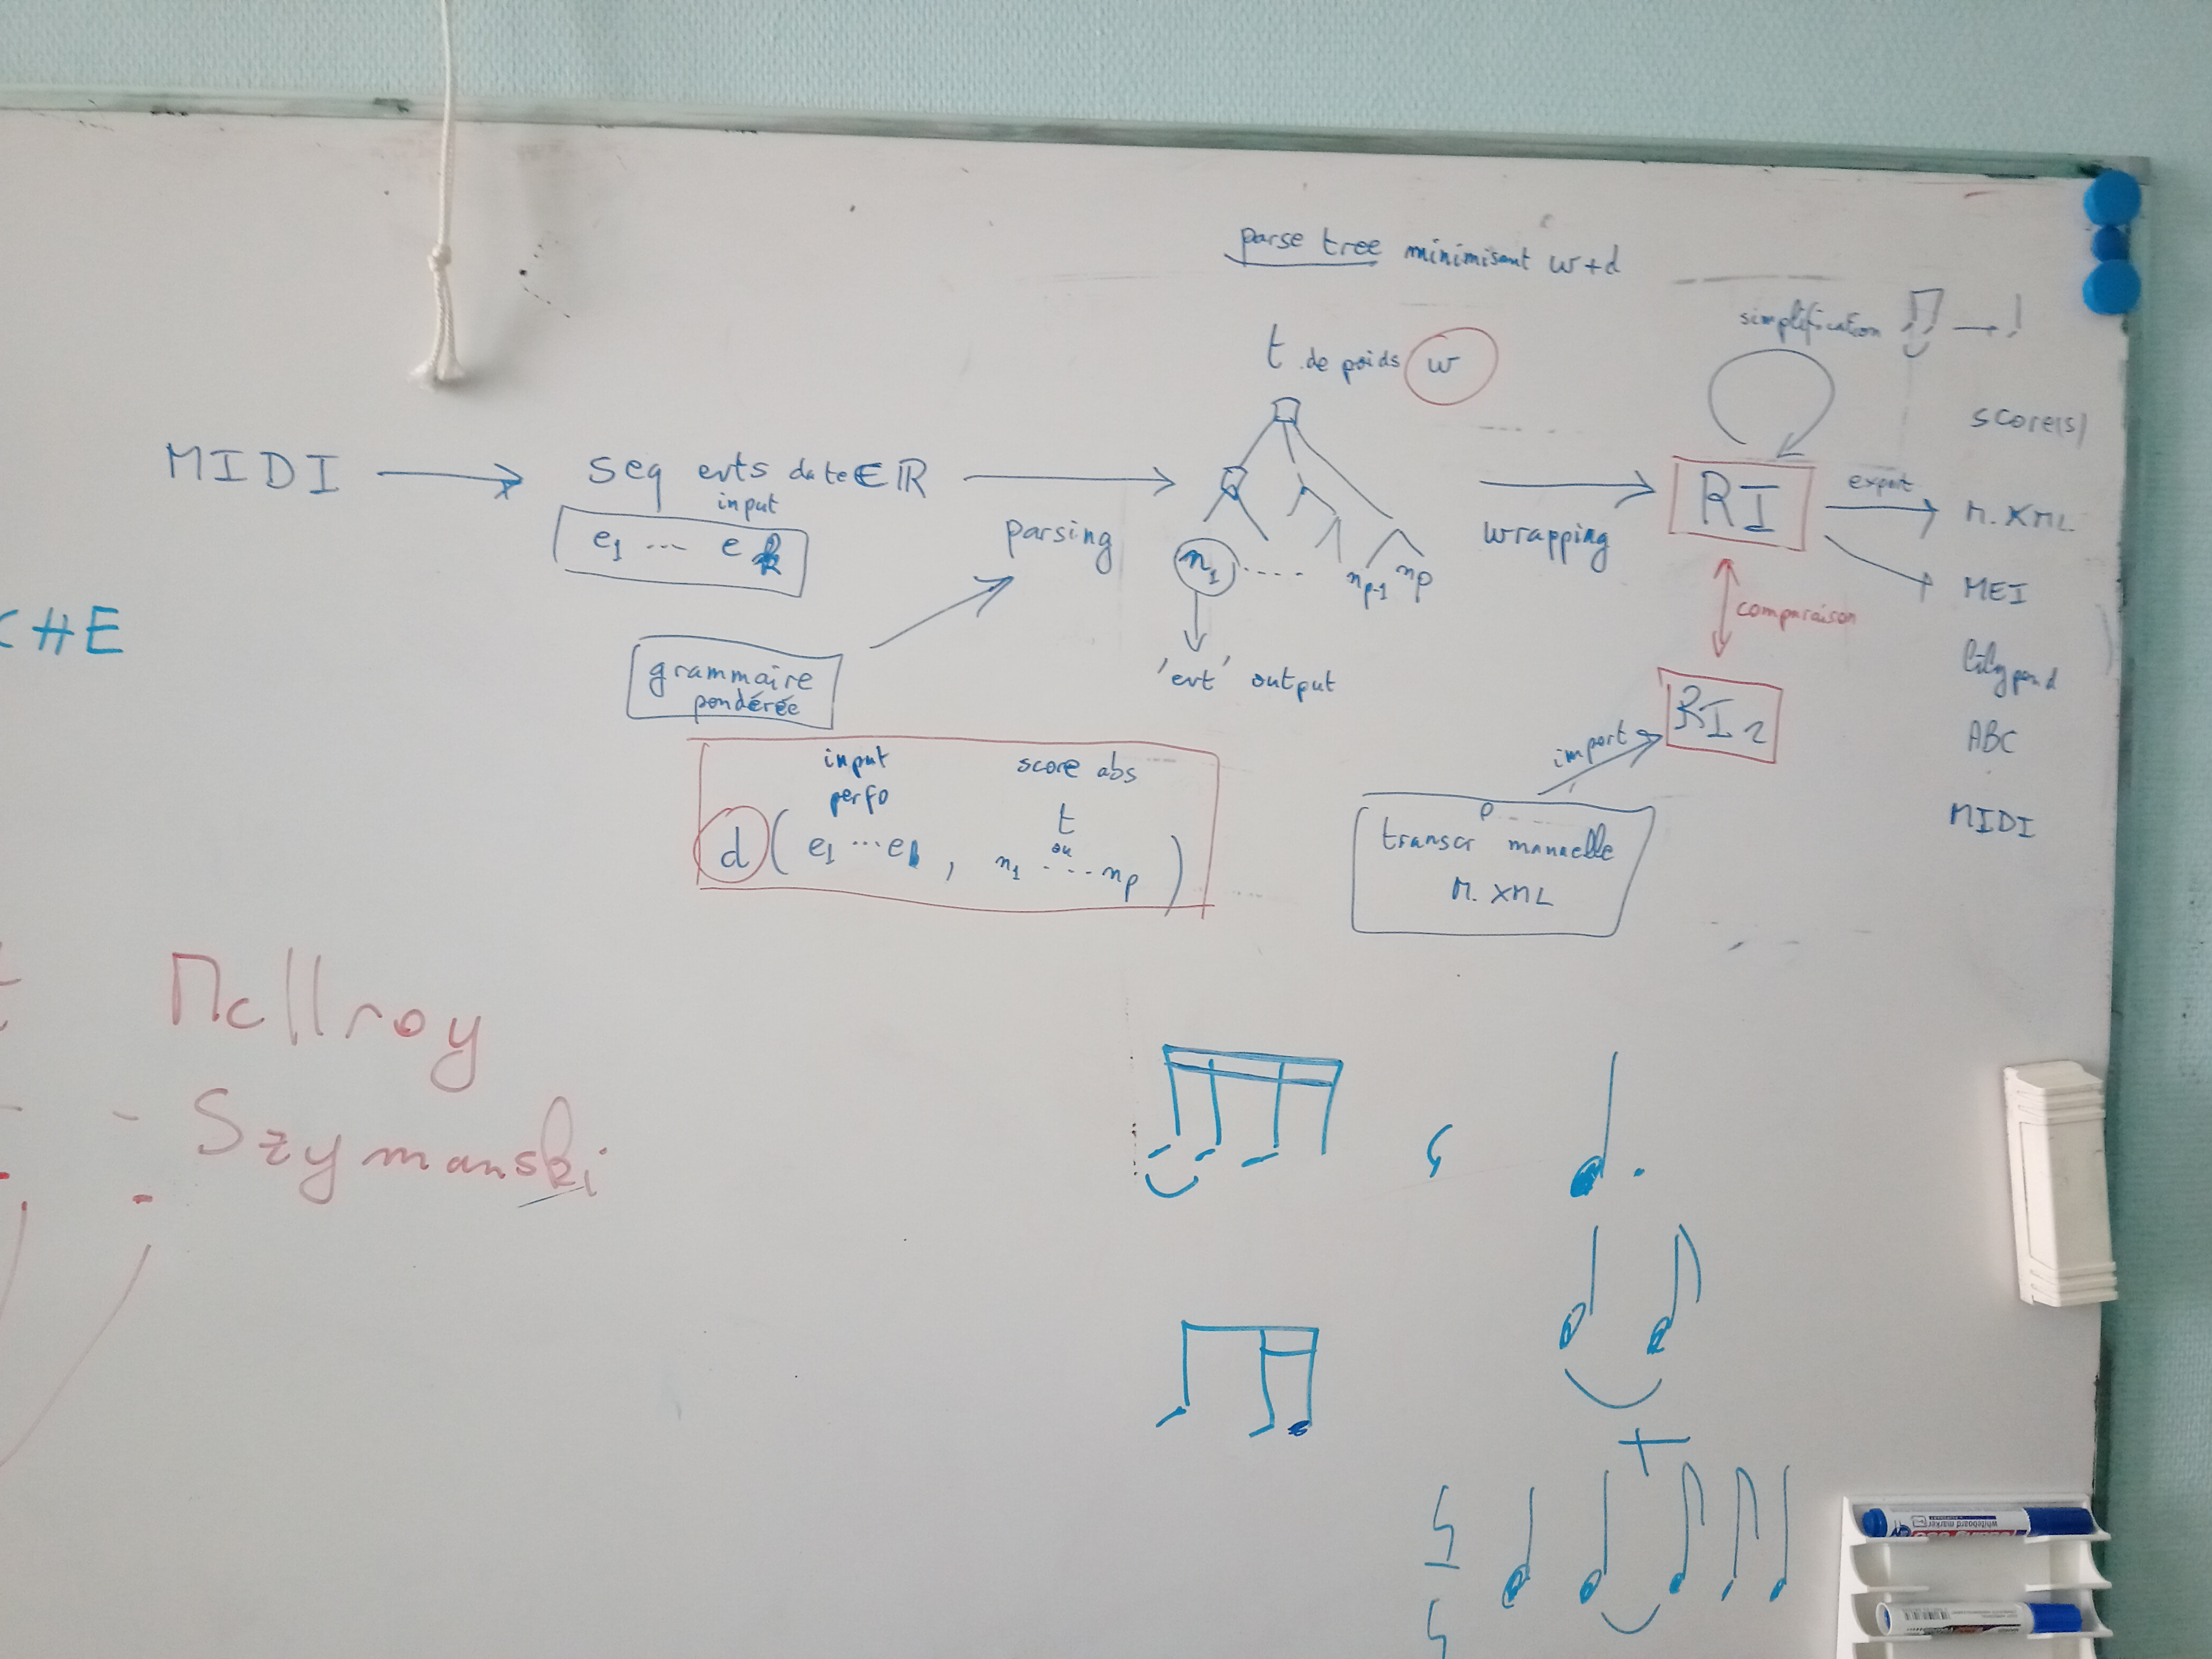
\includegraphics[height=80mm, width=80mm]{images/sujet_stage.jpg} \\\\
	En entrée : midi (séquence d’événements datés (piano roll) accompagné d’une grammaire pondérée)\\
	$\Rightarrow$ parsing\\
	$\Rightarrow$ global parsing tree\\
	$\Rightarrow$ RI (Représentation Intermédiaire) arbres locaux par intruments\\
	$\Rightarrow$ Sortie (xml, mei, lilypond,… )\\
	Minimiser la distance entre le midi et la représentation en arbre.\\\\
	Le but du stage est d’améliorer qparse, un outil de transcription et d’écriture automatique de la batterie (entre autre)\\\\
	\textbf{Le sujet de ce mémoire est de proposer une tâche de reconnaissance du regroupement des notes par les ligatures dans l’écriture de la batterie.}\\\\
	Pour cela, nous utiliserons la logique des systèmes (selon la définition agostinienne).\\$\Rightarrow$ Motif répétitif de plusieurs instruments coordonnées accompagnés d’un texte varié joué par un autre instrument de la batterie.\\\\Nous partirons de propositions génériques de systèmes (environs trois systèmes dans différents style de batterie) que nous tenterons de détecter dans le jeu de données groove.\\\\
	Nous travaillerons aussi sur la détection de répétitions sur plusieurs mesures afin de pouvoir corriger des erreurs sur une des mesures qui aurait dû être identique au autres mais qui présente des différences.
	
	
	

\newpage
\textit{\\En règle générale, l'introduction et la conclusion sont les deux
sections de contenu à ne pas être numérotées. Idéalement, chaque
chapitre commence par une introduction rapide et se termine par une
conclusion rapide pour aider le lecteur à mémoriser et comprendre ce
qui a été fait.}

%%%%%%%%%%%%%%%%%%%%%%%%%%%%%%%%%%%%%%%%%%%%%%%%%%%%%%
%% INTRODUCTION
%%%%%%%%%%%%%%%%%%%%%%%%%%%%%%%%%%%%%%%%%%%%%%%%%%%%%%


\chapter*{Introduction}
\adjustmtc
\addstarredchapter{Introduction} 

\textit{Introduction : présentation générale du contexte et de la
problématique traitée, plan suivi dans le mémoire.}
%% TODO: remplacer ce contenu par le vôtre...
\section*{Pr\'esentation g\'en\'erale}

\subsection*{Sujet du stage}
L'objectif de la transcription automatique de la musique (AMT) [1] est de convertir la performance d'un musicien en notation musicale - un peu comme la conversion de la parole en texte dans le traitement du langage naturel. Elle est considérée comme l'un des problèmes de recherche les plus anciens et les plus difficiles dans le domaine de la recherche d'information musicale (MIR).\\
Le cas de la transcription de la batterie (DT) est très particulier puisqu'il s'agit d'instruments sans hauteur, d'événements avec (presque) aucune durée et de notations spécifiques. Il a été la source de nombreuses études MIR, voir [2] pour un aperçu. La plupart de ces travaux se concentrent sur des méthodes de calcul pour la détection d'événements sonores de batterie à partir de signaux acoustiques, et sur l'extraction de caractéristiques de bas niveau telles que la classe d'instrument et le moment de l'apparition du son (peak picking). Cependant, très peu d'entre eux ont abordé la tâche de générer une notation musicale (rythmique) lisible à partir des caractéristiques ci-dessus, une étape cruciale dans un contexte musical et loin d'être triviale.\\\\
La présente proposition s'intéresse à ce dernier problème, et plus précisément à :

1. l'étude de modèles de langage (LM) incorporant certaines informations musicales de haut niveau nécessaires à la génération de partitions de qualité. On devrait en particulier considérer des hiérarchies d'événements de batterie induisant des placements temporels cohérents et se prêtant à des notations rythmiques faciles à lire pour un batteur entraîné ; voir [3] pour des modèles structurés en arbre basés sur la théorie formelle du langage, que nous développons dans le contexte d'outils AMT plus généraux.\\\\
2. l'intégration de ces LM avec l'état de l'art des modèles acoustiques (AM) et des méthodes pour les tâches de traitement du signal ci-dessus. Cela nécessite la prise en compte du contexte musical et des informations musicales de haut niveau des LM en plus des caractéristiques acoustiques de bas niveau ci-dessus.\\
En outre, certaines expériences seront menées sur la base d'ensembles de données publiques, afin d'évaluer l'approche intégrée. Elles devraient couvrir certains cas de motifs rythmiques complexes se chevauchant.\\

Au-delà de l'intégration de modèles, il sera également intéressant d'étudier comment l'utilisation de LM peut améliorer les résultats de l'AM, voir [2], et ouvrir la voie à la génération entièrement automatisée de partitions de batterie et au problème général de l'AMT de bout en bout.

\subsection*{Problématique traitée}	
	En entrée : midi (séquence d’événements datés (piano roll) accompagné d’une grammaire pondérée)\\
	$\Rightarrow$ parsing\\
	$\Rightarrow$ global parsing tree\\
	$\Rightarrow$ RI (Représentation Intermédiaire) arbres locaux par intruments\\
	$\Rightarrow$ Sortie (xml, mei, lilypond,… )\\
	Minimiser la distance entre le midi et la représentation en arbre.\\\\
	Le but du stage est d’améliorer qparse, un outil de transcription et d’écriture automatique de la batterie (entre autre)\\\\
	Le sujet de ce mémoire est de proposer une tâche de reconnaissance du regroupement des notes par les ligatures dans l’écriture de la batterie.\\\\
	Pour cela, nous utiliserons la logique des systèmes (selon la définition agostinienne).\\$\Rightarrow$ Motif répétitif de plusieurs instruments coordonnées accompagnés d’un texte varié joué par un autre instrument de la batterie.\\\\Nous partirons de propositions génériques de systèmes (environs trois systèmes dans différents style de batterie) que nous tenterons de détecter dans le jeu de données groove.\\\\
	Nous travaillerons aussi sur la détection de répétitions sur plusieurs mesures afin de pouvoir corriger des erreurs sur une des mesures qui aurait dû être identique au autres mais qui présente des différences.
	
\subsection*{Plan suivi dans le mémoire}
\begin{itemize}
	\item écouter le dataset groove
	\item observer la structure midi
	\item décrire la notation de la batterie et transcrire manuellement pour comparer l’input et l’output idéal d’un point de vu théorique.
	\item Détecter les systèmes dans le dataset.
	\item Faire des règles de réécriture (rewriting/simplification) et de séparation des voix (reconnaissance de systèmes)
\end{itemize}
	







%%%%%%%%%%%%%%%%%%%%%%%%%%%%%%%%%%%%%%%%%%%%%%%%%%%%%%%%%%%%%%%%
%% Première partie

\part{Contexte général}



%%%%%%%%%%%%%%%%%%%%%%%%%%%%%%%%%%%%%%%%%%%%%%%%%%%%%%
%% ÉTAT DE L'ART
%%%%%%%%%%%%%%%%%%%%%%%%%%%%%%%%%%%%%%%%%%%%%%%%%%%%%%

%% Nota Bene : il est possible de stocker chaque chapitre dans un
%% fichier *.tex distinct (par exemple pour ce chapitre, de la
%% commande \chapter{} jusqu'à la conclusion de ce chapitre) nommé,
%% par exemple "chapitre-etat-art.tex" qui sera appelé au moyen de la
%% commande suivante (la compilation du fichier *.tex principal
%% compile automatiquement les fichiers inclus) :
%%
%% \include{chapitre-etat-art}

\chapter{\'Etat de l'art}
\label{chap:articles}

%% Ajustement de la mini table des matières du fait de l'introduction
%% non numérotées qui introduit un décalage
\adjustmtc
\minitoc

\textit{\\L’état de l'art (chapitre~\ref{chap:articles})~: les articles
qui traitent du même sujet que vous, présentés en un tout cohérent
\emph{(extraire de chaque article lu les points essentiels et
	présenter dans ce chapitre le résultat de ces lectures en
	regroupant les articles par point essentiel)}}
\section{Introduction}

Dans ce chapitre, nous présentons les différentes avançées qui ont déjà eues lieues dans le domaine de la transcription.

\section{Contenu}
\textbf{Automatic music transcription : Challenges and future directions} \cite{article1}\\
(introduction\cite{article1})\\
\textbf{Les applications de l’AMT ont aussi de la valeur dans les domaine oraux qui manquent de partition (jazz, pop, (et donc batterie, note perso)}\\
(abstract \cite{article1})\\
Les différents travaux existant se préoccupent plus de la transcription à partir de l’audio en passant par le traitement du signal.\\
Les humains sont encore meilleur que les machines et la précisions à l’air d’avoir atteint sa limite.\\
Analyse des limites des méthodes courantes et identification des directions prometteuses.\\
Les modèles généraux utilisés ne traitent pas correctement la riche diversités des signaux musicaux.\\
2 moyens pour surmonter celà :
\begin{itemize}
	\item adapter algo pour des cas d’utilisations spécifiques.
	\item utiliser les approches semi-automatiques.
\end{itemize}
\textbf{La richesse des partitions musicales et des données audio correspondantes, désormais disponibles, constitue une source potentielle de données d'apprentissage, grâce à l'alignement forcé des données audio sur les partitions, mais l'utilisation à grande échelle de ces données n'a pas encore été tentée.}\\
D'autres approches prometteuses incluent l'intégration
d'informations provenant de plusieurs algorithmes et de différents aspects musicaux.
\section{Conclusion}
Conclusion de ce chapitre.
%\section{Introduction}
%Dans ce chapitre, nous présentons...
%
%\section{Contenu}
%Une section dans ce chapitre avec un appel cliquable de référence
%%bibliographique~\cite{grouin-2014jbi}.
%
%\section{Conclusion}
%Conclusion de ce chapitre.


%%%%%%%%%%%%%%%%%%%%%%%%%%%%%%%%%%%%%%%%%%%%%%%%%%%%%%
%% MÉTHODES
%%%%%%%%%%%%%%%%%%%%%%%%%%%%%%%%%%%%%%%%%%%%%%%%%%%%%%


\chapter{Méthodes}
\label{chap:methodes}
\minitoc

\textit{\\Méthodes (chapitre~\ref{chap:methodes})~: les méthodes
appliquées, avec le détail des expériences réalisées (différentes
configurations)~;}

\textit{\\Corpus (chapitre~\ref{chap:corpus})~: le corpus utilisé
	\emph{(caractéristiques, pré-traitements appliqués)}}

\section{Introduction}
Dans ce chapitre...
\subsection{Chaîne de traitement}
\begin{itemize}
	\item Reconnaître un motif (système) dans une partition (un fichier midi)\\
	Sur une mesure de l’input $\Rightarrow$ Motif (système) reconnu : true ou false
	\item Si true : 
	\begin{itemize}
		\item Séparer les voix
		\item Simplifier l’écriture de chaque voix\\\\
	\end{itemize}
\end{itemize}
Chaîne de traitement :\\
if match(system\_parse\_tree(system + pitch), input\_midi\_parse\_tree)\\
\tab then voice\_split ;\\
\tab for voice in voice\_split:\\
\tab \tab simplication voice

\subsection*{Les sytèmes en batterie}
SYSTÈME ==> MOTIF (2-3 instruments sur 1-2 voix, joué en boucle) + TEXTE (1 instrument sur 1 voix, irrégulier)\\
ex : système afro-cubain, trois voix.
Proposition pour la détection de la direction des hampes et pour les ligatures (regroupement des notes et séparation des voix.)
\begin{itemize}
	\item \textbf{\textit{Les systèmes :}}\\
	$\Rightarrow$ Un système est la combinaison d’un ou plusieurs éléments qui jouent un rythme en boucle (système) et d’un autre élément qui joue un \textit{texte} rythmique variable mais respectant les règles propre au système (texte).\\
	Définition d’un système :\\
	
	En cas de système, les ligatures forment deux voies :
	\begin{itemize}
		\item Le texte ;
		\item Le système.
	\end{itemize}
	\textit{Mettre des exemples de différents systèmes.}
	\item \textbf{\textit{Les moulins :}}\\
	Lorsqu’il y a plus d’une voie, ils sont prioritaires pour les ligatures.\\
	\textit{Mettre des exemples.}\\
\end{itemize}
\subsection*{Gestion des silences et des têtes de notes}
Rythme tree (RT)\\
- Le symbole "-" est une continuation (liaison) mais pour une partition de
batterie, ça serait un silence par défaut sauf peut-être pour les ouvertures
de charley et éventuellement les cymbales ou un tom basse qui résonne.\\
$\Rightarrow$ Question de la (notation noir + silence) vs blanche.\\
$\Rightarrow$ On privilégierait (noir + silence) puisque les symboles « x » des cymbales ne
peuvent pas porter d’indication de durée dans la tête de notes.\\
Les 3 parties d’une note :
\begin{itemize}
	\item durée
	\item hampe
	\item tête de note (peut aussi indiquer la durée mais en batterie on évitera les blanches, etc.)
\end{itemize}
source : \url{https://fr.wikipedia.org/wiki/Note_de_musique}\\\\
\subsection*{Définition des têtes de notes et des hauteurs}
\subsubsection*{Proposition de définition d’un standard de départ}
Pour la transcriptions, nous proposons de choisir la base Agostini. La caisse claire centrale sur la portée est aussi centrale sur la batterie est elle est un élément qui conditionne la position des jambes (écart entre les pédales, etc.) ainsi que l’organisation des éléments en hauteur (toms, cymbales, etc.).
On pensera en terme de symétrie la répartition des éléments par rapport au point central que constitue la caisse claire.\\
Cette symétrie s’opère en trois dimensions :
\begin{itemize}
	\item Les hauteurs en terme de fréquences ;
	\item La hauteur physique des éléments :\\
	Du bas vers le haut : pédales, toms et caisse, cymbales
	\item L’ergonomie, qui hiérarchise l’importance des éléments sur la portée (caisse claire au centre, hh-pied et ride sont aux deux extrémités).
\end{itemize}

%\section*{Installation de cmake-3.20.4}
Installation de CMake et d’un environnement C++ pour Vim.\\\\
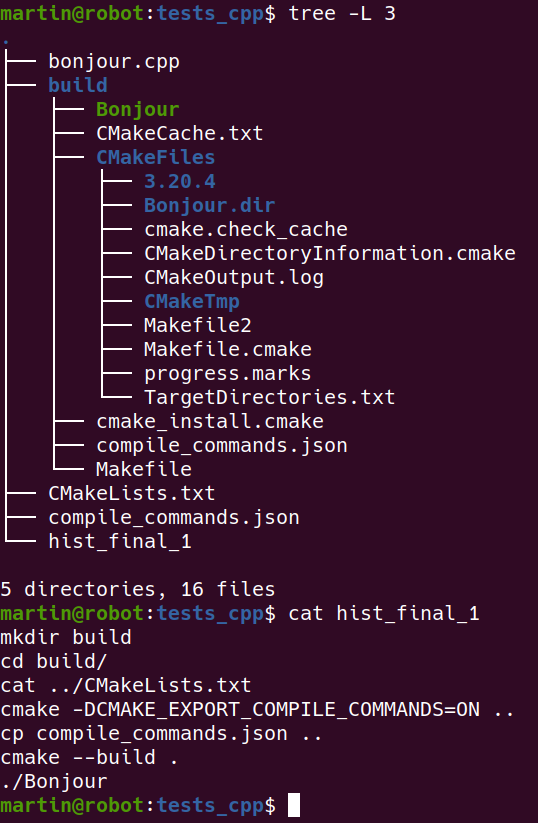
\includegraphics[height=70mm, width=50mm]{images/cpp_env_0.png}\\\\
- Lire sur la réécriture : 1\_articles/1\_rt\_representation\\
- Lire Qparse : \url{https://qparse.gitlabpages.inria.fr/}\\\\
qparse (version beta) entrée MIDI (groove), sortie MIDI (modifiée) ou
partition MEI.
\newpage

\section{Contenu}
\subsection{Caractéristiques pour la représentation et la notation}

\begin{table}[h]
	\centering
	\begin{tabular}{|c|c|c|} \hline
		Pitchs & Instruments \\ \hline
		51 & ride \\
		44 & ch-pf \\
		36 & gc \\
		38 & cc \\
		37 & cross-stick \\ \hline
	\end{tabular}
	\caption{Pitchs et instruments}
	%	\label{tab:exemple}
\end{table}
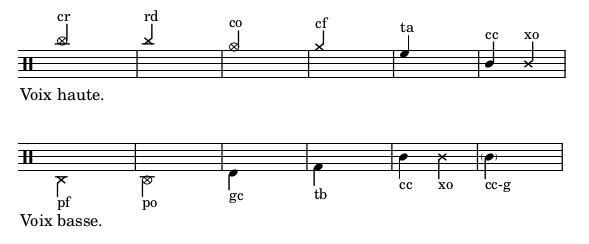
\includegraphics[height=65mm, width=150mm]{images/description_notation/description_notation.png}\\\\
La vélocité sera une donnée importante pour reconnaître les ghosts-notes.\\ Par exemple, pour la caisse-claire, un coup normal (after-beat) monte au dessus de 70 et une ghost-note est autour de 30.
\subsection{Les systèmes}
Créer un ensemble de systèmes :
\begin{itemize}
\item Trouver les systèmes intéressants dans groove ;
\item Compléter avec des systèmes ago personnalisés ;
\item Tout transcrire avec lilypond et en arbres d’analyse syntaxique.
\item Créer les arbres de voix séparées.
\item Créer les arbres de voix séparées simplifiés (rewriting).\\	
\end{itemize}

%preamble:
%
%
%%\usetikzlibrary{backgrounds}
%%\usetikzlibrary{trees}
%
%
%Figure 1:
%
%\begin{figure}
%\centering
%\subfigure
%[$\frac{1}{2} \frac{1}{4} \frac{1}{4}$]
%{
%\begin{tabular}{c}
%%\includegraphics[scale=\scorescale]{images/1a.png}\\
%\begin{tikzpicture} [-,thick]
%\tikzstyle{level 1}=[level distance=7mm,sibling distance=6mm]
%\tikzstyle{level 2}=[level distance=7mm,sibling distance=5mm]
%\node {$\deux$}
%  child { node {$\note$} }
%  child { node {$\deux$}
%    child { node {$\note$} }
%    child { node {$\note$} } };
%\end{tikzpicture}
%\end{tabular}
%\label{fig:subfig1a}}
%%
%\hspace{0.6cm}
%\subfigure
%[$\lbrack \frac{1}{6} \rbrack\, \frac{1}{6}\,
%  \lbrack \frac{1}{6} \rbrack\, \frac{1}{6}\,
%  \lbrack \frac{1}{6} \rbrack\, \frac{1}{6}$]
%{
%\begin{tabular}{c}
%%\includegraphics[scale=\scorescale]{images/1b.png}\\
%\begin{tikzpicture} [-,thick]
%\tikzstyle{level 1}=[level distance=7mm,sibling distance=9mm]
%\tikzstyle{level 2}=[level distance=7mm,sibling distance=5mm]
%\node {$\trois$}
%  child { node {$\deux$}
%    child { node {$\rest$} }
%    child { node {$\note$} } }
%  child { node {$\deux$}
%    child { node {$\rest$} }
%    child { node {$\note$} } }
%  child { node {$\deux$}
%    child { node {$\rest$} }
%    child { node {$\note$} } };
%\end{tikzpicture}
%\end{tabular}
%\label{fig:subfig1b}}
%%
%\hspace{0.6cm}
%\subfigure
%[$\frac{1}{5} \frac{1}{5}
%  \frac{1}{15}\frac{1}{15}\frac{1}{15}
%  \frac{1}{5} \frac{1}{5}$]
%{
%\begin{tabular}{c}
%%\includegraphics[scale=\scorescale]{images/1c.png}\\
%\begin{tikzpicture} [-,thick]
%\tikzstyle{level 1}=[level distance=7mm,sibling distance=5mm]
%\tikzstyle{level 2}=[level distance=7mm,sibling distance=5mm]
%\node {$\cinq$}
%  child { node {$\note$} }
%  child { node {$\note$} }
%  child { node {$\trois$}
%    child { node {$\note$} }
%    child { node {$\note$} }
%    child { node {$\note$} } }
%  child { node {$\note$} }
%  child { node {$\note$} } ;
%\end{tikzpicture}
%\end{tabular}
%\label{fig:subfig1c}}
%%
%\begin{RR}
%\hspace{0.6cm}
%\subfigure
%[$\frac{1}{12} \frac{1}{12} \frac{1}{12} \frac{1}{12} \frac{1}{3}
%\frac{1}{12} \frac{1}{12} \frac{1}{12} \frac{1}{12}$]
%{
%\begin{tabular}{c}
%%\includegraphics[scale=0\scorescale]{images/1d.png}\\
%%\hspace{0.3cm}
%\begin{tikzpicture} [-,thick]
%\tikzstyle{level 1}=[level distance=7mm,sibling distance=9mm]
%\tikzstyle{level 2}=[level distance=6mm,sibling distance=8mm]
%\tikzstyle{level 3}=[level distance=6mm,sibling distance=5mm]
%\node {$\trois$}
%  child { node {$\deux$}
%    child { node {$\deux$}
%      child { node {$\note$} }
%  child { node {$\note$} } }
%    child { node {$\deux$}
%      child { node {$\note$} }
%  child { node {$\note$} } } }
%  child { node {$\note$} }
%  child { node {$\deux$}
%    child { node {$\deux$}
%      child { node {$\note$} }
%  child { node {$\note$} } }
%    child { node {$\deux$}
%      child { node {$\note$} }
%  child { node {$\note$} } } };
%\end{tikzpicture}
%\end{tabular}
%\label{fig:subfig1d}}
%\end{RR}
%\caption{Simple trees of $\T(\Sigmar)$ with their corresponding
%rhythmic notations and values.}
%\label{fig:trees0}
%\end{figure}
%\subsection*{Tests avec qtree}
[…]\\

%\Tree[.IP [.NP [.Det \textit{the} ]
%               [.N\1 [.N \textit{package} ]]]
%          [.I\1 [.I \textsc{3sg.Pres} ]
%                [.VP [.V\1 [.V \textit{is} ]
%                           [.AP [.Deg \textit{really} ]
%                                [.A\1 [.A \textit{simple} ]
%                                      \qroof{\textit{to use}}.CP ]]]]]]
%                                      
%\Tree[. [. [.rd\\gc ][. [rd\\chpf ][rd ]]]
%        [. [.rd\\cc ][. [rd\\chpf ][rd ]]]
%        [. [.rd\\gc ][. [rd\\chpf ][rd ]]]
%        [. [.rd\\cc ][. [rd\\chpf ][rd ]]] ]
%Voix haute (Les mesure 1 et 2 sont identiques) :\\\\
%\Tree[. [. [rd ][. [rd ][rd ]]]
%        [. [rd\\cc ][. [rd ][rd ]]]
%        [. [rd ][. [rd ][rd ]]]
%        [. [rd\\cc ][. [rd ][rd ]]] ]\\\\\\
%Voix basse (mesure 1) :
%\Tree[. [. [gc ][. [pf ][$\emptyset$ ]]]
%        [. [$\emptyset$ ][. [pf ][$\emptyset$ ]]]
%        [. [gc ][. [pf ][$\emptyset$ ]]]
%        [. [$\emptyset$ ][. [pf ][$\emptyset$ ]]] ]\\
%Voix basse (mesure 2) :
%\Tree[. [. [$\emptyset$ ][. [pf\\gc ][$\emptyset$ ]]]
%		[. [$\emptyset$ ][. [pf\\gc ][$\emptyset$ ]]]
%		[. [$\emptyset$ ][. [pf\\gc ][$\emptyset$ ]]]
%		[. [$\emptyset$ ][. [pf\\gc ][$\emptyset$ ]]] ]\\\\\\
%\resizebox{420pt}{!}{\Tree[.Voix\ haute 
%	[.Mesure\ 1 
%			[. [rd ][. [rd ][rd ]]]
%			[. [rd\\cc ][. [rd ][rd ]]]
%			[. [rd ][. [rd ][rd ]]]
%			[. [rd\\cc ][. [rd ][rd ]]] ]
%	[.Mesure\ 2 
%			[. [rd ][. [rd ][rd ]]]
%			[. [rd\\cc ][. [rd ][rd ]]]
%			[. [rd ][. [rd ][rd ]]]
%			[. [rd\\cc ][. [rd ][rd ]]] ]]}
%\resizebox{420pt}{!}{\Tree[.Voix\ basse 
%	[.Mesure\ 1 
%	       [. [gc ][. [pf ][$\emptyset$ ]]]
%	       [. [$\emptyset$ ][. [pf ][$\emptyset$ ]]]
%	       [. [gc ][. [pf ][$\emptyset$ ]]]
%	       [. [$\emptyset$ ][. [chpf ][$\emptyset$ ]]] ]
%	[.Mesure\ 2 
%	       [. [$\emptyset$ ][. [pf\\gc ][$\emptyset$ ]]]
%	       [. [$\emptyset$ ][. [pf\\gc ][$\emptyset$ ]]]
%	       [. [$\emptyset$ ][. [pf\\gc ][$\emptyset$ ]]]
%	       [. [$\emptyset$ ][. [pf\\gc ][$\emptyset$ ]]] ]]}
%\Tree[. [. [.rd\\gc ][. [rd\\chpf ][rd ]]]
%        [. [.rd\\cc ][. [rd\\chpf ][rd ]]]
%        [. [.rd\\gc ][. [rd\\chpf ][rd ]]]
%        [. [.rd\\cc ][. [rd\\chpf ][rd ]]] ]
%\Tree[. [. [.51\\36 ][. [51\\44 ][51 ]]]
%[. [.51\\38 ][. [51\\44 ][51 ]]]
%[. [.51\\36 ][. [51\\44 ][51 ]]]
%[. [.51\\38 ][. [51\\44 ][51 ]]] ]

%\resizebox{420pt}{!}{\Tree[.Système [.Mesure\ 1  [.Temps\ 1 [.51\\36 ][. [51\\44 ][51 ]]]
%		   [.Temps\ 2 [.51\\38 ][. [51\\44 ][51 ]]]
%		   [.Temps\ 3 [.51\\36 ][. [51\\44 ][51 ]]]
%		   [.Temps\ 4 [.51\\38 ][. [51\\44 ][51 ]]] ]
%		[.Mesure\ 2 [.Temps\ 1 [.51 ][. [51\\44\\36 ][51 ]]]
% 		   [.Temps\ 2 [.51\\38 ][. [51\\44\\36 ][51 ]]]
%           [.Temps\ 3 [.51 ][. [51\\44\\36 ][51 ]]]
%           [.Temps\ 4 [.51\\38 ][. [51\\44\\36 ][51 ]]] ]]}

% L’arbre est trop grand, autre technique que resizebox à ce lien :
% https://tex.stackexchange.com/questions/336314/resizing-qtree-to-fit-pagewidth
\subsubsection*{Propositions de règles de ré-écriture}
Basé sur \cite{jacquemard:hal-01134096} et sur \cite{jacquemard:hal-01403982}
Pour la plupart des instruments mélodiques, la liaison et le point sont les deux seules possibilités en cas d’équivalence rythmique. Mais la batterie offre un 3ème choix pour combler la distance rythmique entre deux notes : les silences.\\Les cymbales-crash et les ouvertures de charley constituent le seul cas qui exclut cette option. Le charley car ses ouvertures/fermetures sont presque toujours quantifiées. Les fermetures du charley sont notées soit par un silence (correspondant à une fermeture de la pédale), soit par un écrasement de l’ouverture par un autre coup de charley fermé, au pied ou à la main.
\begin{itemize}
\item 
Tie to dot devient Tie to note\&rest\\
par exemple : une noire liée à une autre noire devient une noire + un soupir.\\
On remplace donc la dernière note d’une liaison par sa valeur en silence.
Ceci ne concerne pas les ouvertures de charley, qui sont, avec les cymbales-crash, les seuls indications sonores dont nous considèrerons la durée.
\item 
Dans tous les cas, sauf ouverture de hh-pd, Une note sur un temps suivie d’une note en l’air sur le second temps seront écrites : noire sur le temps 1 puis silence + note pertinente sur le temps 2.
\item
Pour un charley ouvert qui déborde sur le temps d’après, le choix le plus pertinent est-il la note pointée ou la liaison ? Je pense que c’est la liaison car il marchera même dans les cas où le point ne marche pas (ex : mauvaise durée)
\item
une blanche sera écrite noir + soupir.\\
Voir exemples dans :
Stage\_M2\_Inria/2\_Transcriptions\_LilyPond/exemples\_rewriting
\end{itemize}


\section{Conclusion}
Conclusion de ce chapitre.


%%%%%%%%%%%%%%%%%%%%%%%%%%%%%%%%%%%%%%%%%%%%%%%%%%%%%%%%%%%%%%%%
%% Deuxième partie

\part{Expérimentations}



%%%%%%%%%%%%%%%%%%%%%%%%%%%%%%%%%%%%%%%%%%%%%%%%%%%%%%
%% CORPUS
%%%%%%%%%%%%%%%%%%%%%%%%%%%%%%%%%%%%%%%%%%%%%%%%%%%%%%


\chapter{Corpus}
\label{chap:corpus}
\minitoc

\section{Introduction}
Dans ce chapitre...
\textbf{groove MIDI dataset}\\
	\url{https://magenta.tensorflow.org/datasets/groove}\\\\
	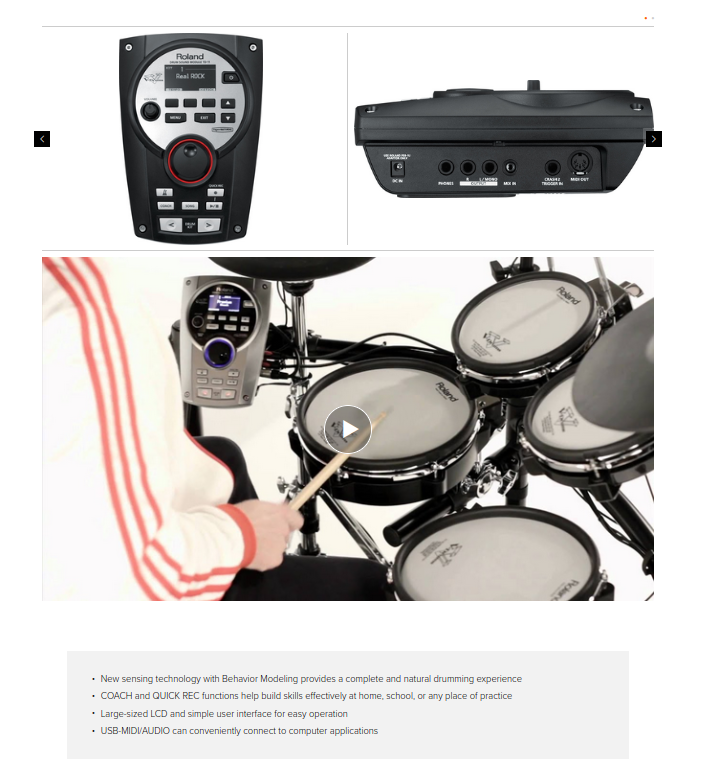
\includegraphics[height=60mm, width=60mm]{images/presentation_groove/roland_TD11.png}\\
	Des batteurs pro ont été engagés pour jouer sur un roland td-11\\\\
	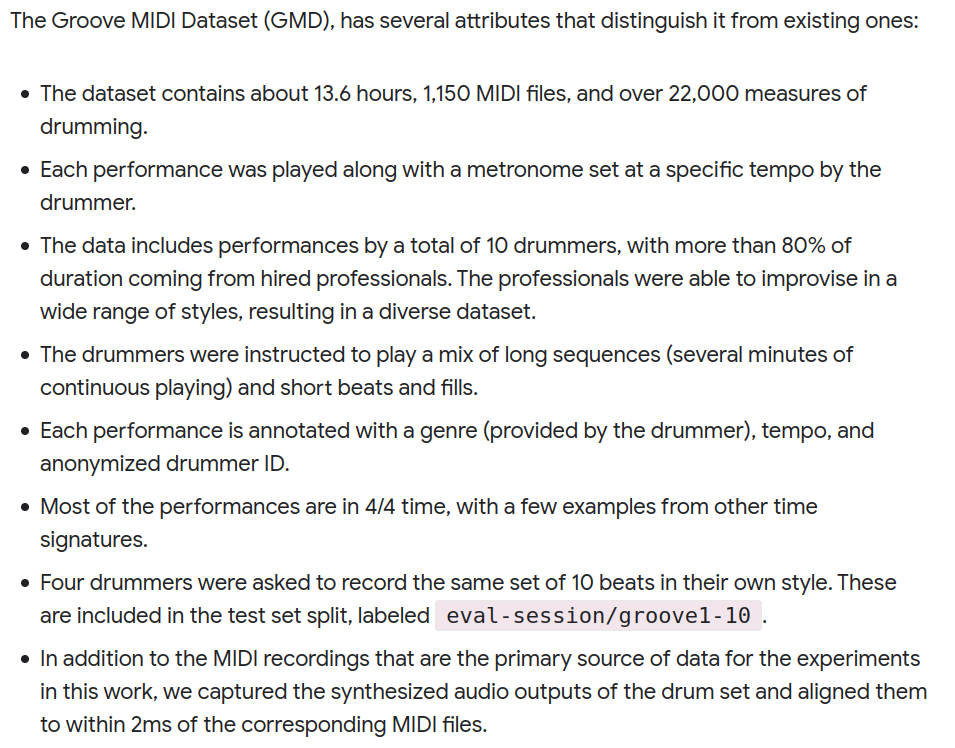
\includegraphics[height=80mm, width=110mm]{images/presentation_groove/dataset_how.png}\newpage{}
	\textbf{Les métadatas :}\\\\
	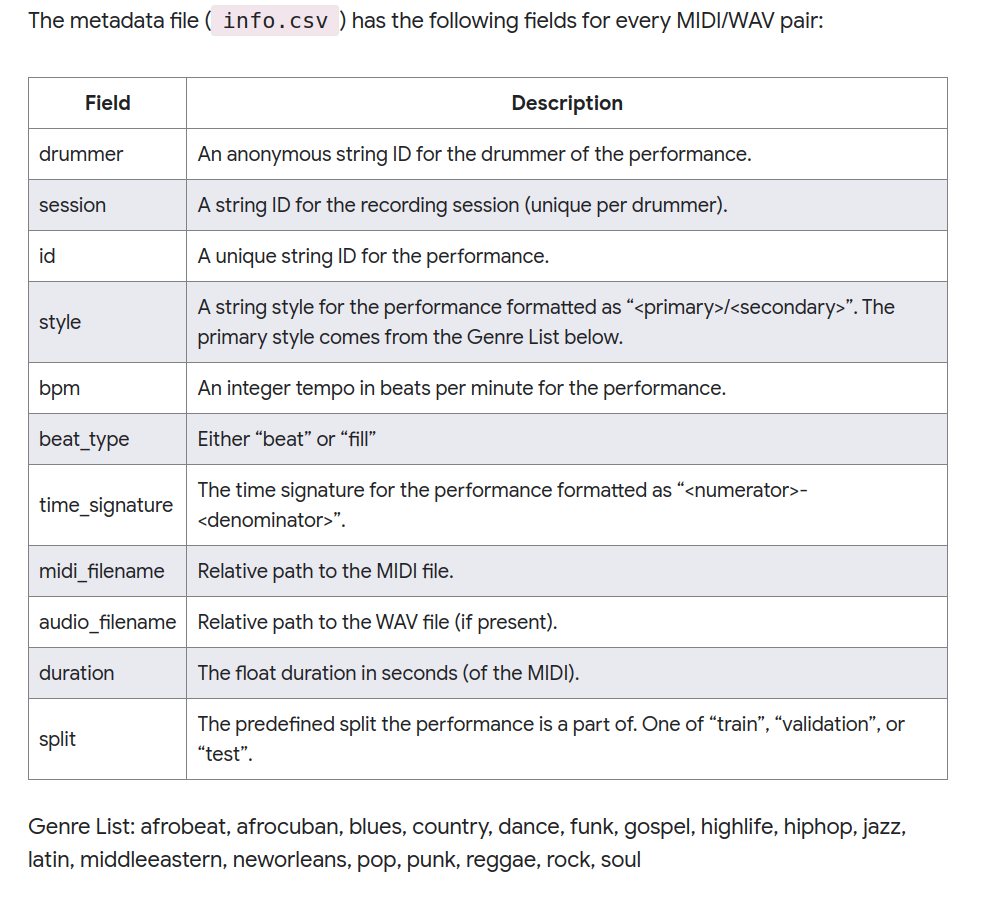
\includegraphics[height=85mm, 
	width=100mm]{images/presentation_groove/csv_metadata_struct.png}\\
	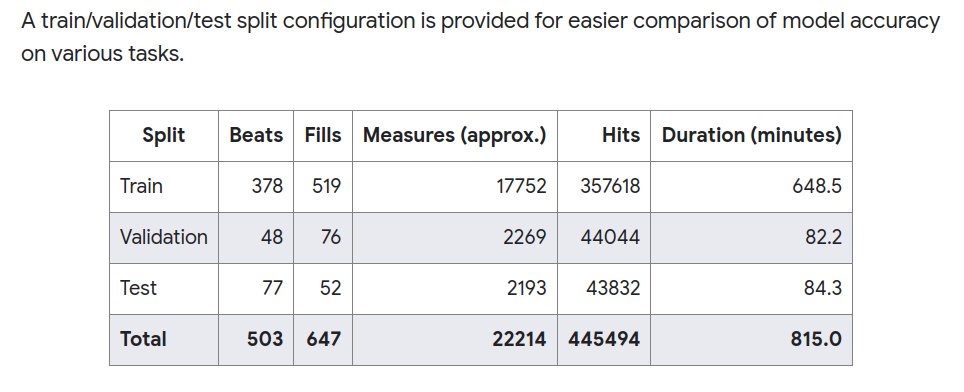
\includegraphics[height=50mm, width=120mm]{images/presentation_groove/train_validation_test.png}\\
	Détails (entre autres tensorflow avec le dataset) à :
	\url{https://magenta.tensorflow.org/datasets/groove#license}\\
	\newpage
%Les transcriptions manuelles sont faites à partir des fichiers wav et celles de MuseScore à partir des fichiers MIDI.\\
\section{Partitions entières}
Mettre ici des partitions entièrement transcrites.
\section{Comparaisons de transcriptions}
\subsection*{0. Prise en main}
Pour la prise en main, les transcriptions manuelles ont été faites avec musescore au lieu de lilypond.
\textbf{Premiers tests sur drummer\_01/session3}\\

\textbf{\textit{Exemple 1 : 10\_rock-folk\_90\_beat\_4-4}}\\\\
\textbf{manuelle}\\
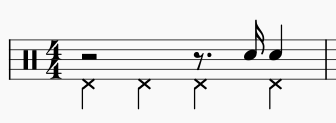
\includegraphics[height=25mm, width=70mm]{images/transcriptions_manuelles/0_prise_en_main/0_tests_drummer_01__session3/manuel_0.png} \\
\textbf{musescore}\\
\includegraphics[height=25mm, width=70mm]{images/transcriptions_manuelles/0_prise_en_main/0_tests_drummer_01__session3/musescore_0.png} \\
\begin{itemize}
	\item Erreur d’indication de mesure ;
	\item Mauvaise transcription d’une noire.\\
\end{itemize}
La noire du 4ème temps se retrouve sur le premier temps de la mesure suivante et elle se transforme en un triolet de double croches dont seules les deux premières seraient jouées.\\\\
\textbf{\textit{Exemple 2 : 10\_rock-folk\_90\_beat\_4-4}}\\\\
\textbf{manuelle}\\
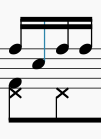
\includegraphics[height=30mm, width=25mm]{images/transcriptions_manuelles/0_prise_en_main/0_tests_drummer_01__session3/manuel_1.png} \\
\textbf{musescore}\\
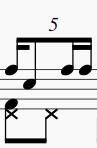
\includegraphics[height=30mm, width=25mm]{images/transcriptions_manuelles/0_prise_en_main/0_tests_drummer_01__session3/musescore_1.png} \\
\begin{itemize}
	\item Erreur de quantification : les doubles croches ont été interprétées en quintolet;\\
\end{itemize}
\textbf{\textit{Exemple 3 : 2\_jazz-swing\_185\_beat\_4-4}}
\\\\
\textbf{manuelle}\\
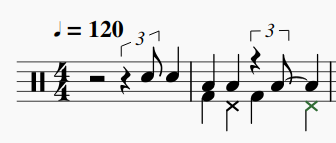
\includegraphics[height=30mm, width=65mm]{images/transcriptions_manuelles/0_prise_en_main/0_tests_drummer_01__session3/manuel_2.png} \\
\textbf{musescore}\\
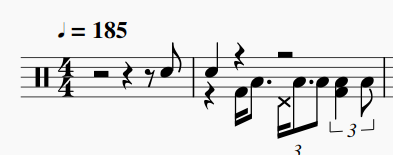
\includegraphics[height=30mm, width=65mm]{images/transcriptions_manuelles/0_prise_en_main/0_tests_drummer_01__session3/musescore_2.png} \\
\begin{itemize}
	\item L’indication de mesure est correcte mais tout a été décalé d’un temps car la première noire sur la caisse claire est jouée sur le 4ème temps et non sur le premier temps de la deuxième mesure comme l’indique la transcription de musescore.
	\item Les toms basses des 1er et 2ème temps de la mesure musescore auraient dû être sur les temps et non décalés d’une double croche vers la droite.\\
\end{itemize}
\textbf{Solutions aux pb rencontrés}\\\\
Existe-t-il un moyen de rectifier les erreurs d’indication de mesure et de décalage de temps des partitions MuseScores.\\
\begin{itemize}
	\item Changer dans manuellement dans MuseScore l’indication de mesure\footnote{\url{https://musescore.org/fr/manuel/indications-de-mesure}} fonctionne avec la transcription du MIDI. \\\\ 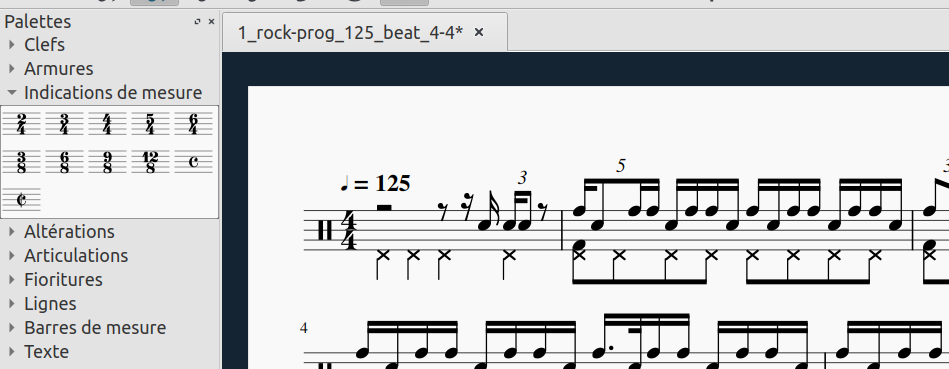
\includegraphics[height=30mm, width=65mm]{images/transcriptions_manuelles/0_prise_en_main/0_tests_drummer_01__session3/solution_0.png} \\
	\item Pour décaler tout d’un temps, on peut sélectionner les mesures en question en cliquant sur la première note de la séquence et en maj-cliquant sur la dernière, puis Ctrl-X Ctrl-V pour replacer le tout au bon endroit.\footnote{\url{https://musescore.org/fr/node/276292}}\\
\end{itemize}

\textit{À partir de la prochaine section, les indications de mesures erronées ou les décalages de temps qui ont des répercussions sur l’ensemble de la partition seront corrigés avant l’analyse.}\\\\
\textbf{Seconds tests sur drummer\_01/session1}\\\\
\textbf{\textit{Exemple 1 : 1\_funk\_80\_beat\_4-4}}
\textbf{manuelle}\\
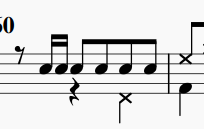
\includegraphics[height=25mm, width=40mm]{images/transcriptions_manuelles/0_prise_en_main/1_drummer_01__session1/Manuelle_0.png} \\
\textbf{musescore}\\
\includegraphics[height=25mm, width=40mm]{images/transcriptions_manuelles/0_prise_en_main/1_drummer_01__session1/musescore_0.png} \\
\begin{itemize}
	\item On dirait que lorsque certaines notes sont proches, elles se resserrent et suppriment celles qui aurait dû être sur le temps.\\
\end{itemize}
\textbf{\textit{Exemple 2 : 1\_funk\_80\_beat\_4-4}}
1\_funk\_80\_beat\_4-4\\\\
\textbf{manuelle}\\
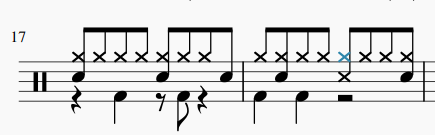
\includegraphics[height=25mm, width=70mm]{images/transcriptions_manuelles/0_prise_en_main/1_drummer_01__session1/Manuelle_1.png} \\
\textbf{musescore}\\
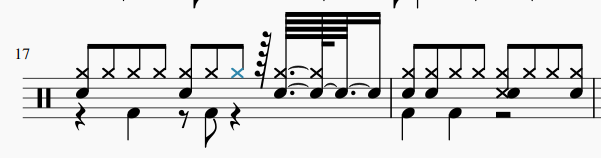
\includegraphics[height=25mm, width=70mm]{images/transcriptions_manuelles/0_prise_en_main/1_drummer_01__session1/MuseScore_1.png} \\
\begin{itemize}
	\item La caisse claire de la 2ème croche du 4ème temps de la 1ère mesure se transforme en une combinaison de quadruple/quintuple/double croches liées qui commence par un soupir et finit en débordant sur le premier temps de la mesure suivante. 
\end{itemize}
\newpage
\subsection*{1. Transcription des flas}
À partir de maintenant, les transcriptions manuelles seront faites avec LilyPond.
\subsubsection{Sur la question des flas}
Des exemples de notation flas tom/caisse-claire existent dans des partitions récentes (rythmique binaire J.-F. Juskowiak).\\
$\Rightarrow$ Ils faudra donc les prendre en compte dans les comparaisons de transcriptions.
De gauche à droite : transcription musescore, transcription manuelle.\\
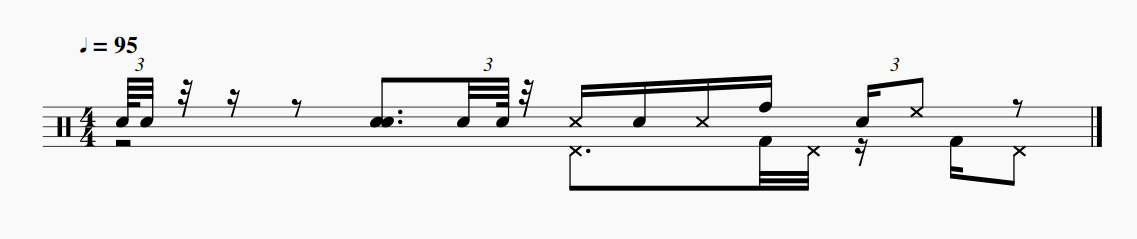
\includegraphics[height=20mm, width=80mm]{images/transcriptions_manuelles/1_transcriptions_flas/124_funk_95_fill_4-4_0.png}
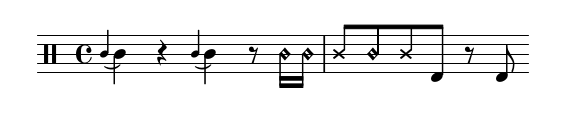
\includegraphics[height=20mm, width=80mm]{images/transcriptions_manuelles/1_transcriptions_flas/124_funk_95_fill_4-4_1.png}\\
Il manque des charley, je dois trouver comment faire des accords avec des têtes de notes différentes.\\\\
\subsection*{2. Autres}
- Chercher des exemples de silences, tuplets.\\
- Faire les observations avec des notations plus ou moins chargées.

\section{Contenu}
Une section dans ce chapitre...

\section{Conclusion}
Conclusion de ce chapitre.


%%%%%%%%%%%%%%%%%%%%%%%%%%%%%%%%%%%%%%%%%%%%%%%%%%%%%%
%% RÉSULTATS
%%%%%%%%%%%%%%%%%%%%%%%%%%%%%%%%%%%%%%%%%%%%%%%%%%%%%%

\chapter{Résultats}
\label{chap:resultats}
\minitoc

\textit{\\Résultats (chapitre~\ref{chap:resultats})~: les résultats
obtenus sur chacune des expériences~;}

\section{Introduction}
Dans ce chapitre...

\section{Contenu}
Une section dans ce chapitre...

\section{Conclusion}
Conclusion de ce chapitre.


%%%%%%%%%%%%%%%%%%%%%%%%%%%%%%%%%%%%%%%%%%%%%%%%%%%%%%
%% DISCUSSION
%%%%%%%%%%%%%%%%%%%%%%%%%%%%%%%%%%%%%%%%%%%%%%%%%%%%%%

\chapter{Discussion}
\label{chap:discussion}
\minitoc

\textit{\\Discussion (chapitre~\ref{chap:discussion})~: la discussion des
résultats obtenus (quelle expérience a produit les meilleurs
résultats, de manière globale, dans le détail des catégories) avec,
si possible, une analyse des erreurs pour comprendre les
possibilités d'amélioration~;}

\section{Introduction}
Dans ce chapitre...

\section{Contenu}
Une section dans ce chapitre...

\section{Conclusion}
Conclusion de ce chapitre.


%%%%%%%%%%%%%%%%%%%%%%%%%%%%%%%%%%%%%%%%%%%%%%%%%%%%%%
%% CONCLUSION
%%%%%%%%%%%%%%%%%%%%%%%%%%%%%%%%%%%%%%%%%%%%%%%%%%%%%%

\cleardoublepage\pdfbookmark[-1]{Conclusion générale}{conclusion} %% CG: lien dans le PDF hors d'une partie
\chapter*{Conclusion générale}
\adjustmtc
\addstarredchapter{Conclusion générale}
\textit{\\Conclusion~: la conclusion globale du mémoire.}\\\\
Dans ce mémoire, nous avons traité de la problématique...


% ================================== BIBLIOGRAPHIE =============================

\cleardoublepage\pdfbookmark[-1]{Bibliographie}{bibliography}
%\selectlanguage{english}
 
\bibliographystyle{unsrt} % Les entrées sont disposées selon leur ordre d’apparition dans la base de donnée bibliographique et étiquetées par un numéro entre crochets.
\bibliography{biblio} % pour afficher la biblio
%\selectlanguage{french} 

\appendix
\cleardoublepage\pdfbookmark[-1]{Annexes}{appendix}
%% TODO: mettre en commentaires les annexes, ou remplacer l'appel de
%% fichier *.tex par votre fichier d'annexe.
\chapter{lilypond}
\section*{Écriture de partitions}
Les partitions pour la description des systèmes et les transcriptions manuelles sont écrites avec LilyPond.\\\\
Le fichier description\_notation.ly :
\begin{verbatim}
\version "2.22.1"
\language français
\include "../0_drum_style_perso.ly"

up = {
\clef percussion
\override Staff.TimeSignature.stencil = ##f
\x do''4-"rd" s s s \c la'4-"co" s s s \x la'4-"cf" s s s \o fa'4-"ta" s s s do'-"cc" s s s \x do'-"xo" s s s
}
down = {
\clef percussion
\override Staff.TimeSignature.stencil = ##f
s s s s s
}
\score 
{
<<
\new Staff
<<
\new Voice { \voiceOne \up }
\new Voice { \voiceTwo \down }
>>
\addlyrics { "Voix haute." }
>>
}

up = {
\clef percussion
\override Staff.TimeSignature.stencil = ##f
s s s s s
}
down = {
\clef percussion
\override Staff.TimeSignature.stencil = ##f
\x do4-"pf" s s s \c do4-"po" s s s \o mi-"gc" s s s sol-"tb" s s s do'-"cc" s s s \x do'-"xo" s s s
}
\score 
{
<<
\new Staff
<<
\new Voice { \voiceOne \up }
\new Voice { \voiceTwo \down }
>>
\addlyrics { "Voix basse." }
>>
}
\end{verbatim}
Et le fichier 0\_drum\_style\_perso.ly :
\begin{verbatim}
\version "2.22.1"
\language français

% LES TÊTES DE NOTES

% Standards noteheads
o = {
\revert NoteHead.style
}

% Cymbales, HH, or cross-stick
x = {
\override NoteHead.style = #'cross
}

% Open HH
c = {
\override NoteHead.style = #'xcircle
}

% Ghost notes
g = {
\override NoteHead.style = #'harmonic
}

% Caisse claire : \o + do'
% Cross stick : \x + do'
% Grosse caisse : \o + mi
% Ride : \x + do''
% Charley : \x + la'
% Charley ouvert : \c + la'
% Charley au pied : \x + do
% Charley ouvert au pied : \c + do

% FLAS

% Flas caisse-claire
fla_cc = {
\appoggiatura do'8 do'4
}
\end{verbatim}
Ces scripts génèrent le document suivant :\\
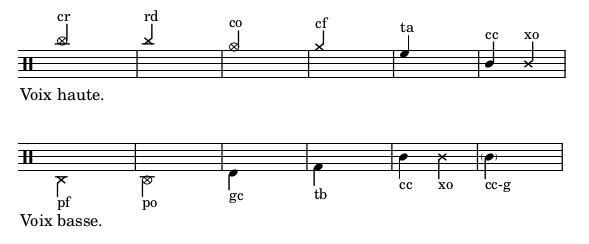
\includegraphics[height=50mm, width=110mm]{images/description_notation/description_notation.png}\\\\
\textbf{Bases :}\\
\url{http://lilypond.org/doc/v2.22/Documentation/learning/simple-notation}\\

\textbf{Percussions et batterie :}\\
\url{http://lilypond.org/doc/v2.22/Documentation/notation/common-notation-for-percussion}\\


\documentclass{report}
\usepackage[pagebackref,colorlinks=true,citecolor=forestgreen,linkcolor=black,menucolor=alezan]{hyperref}
\begin{document}
\chapter{Principes à suivre}

\section{Le sujet de votre mémoire}
Vous avez acquis, au cours de l'année 2015-2016, des compétences d'ingénieur-linguiste ; vous savez donc analyser un problème, proposer une méthodologie permettant d'arriver à une solution et montrer les limites de cette dernière. C'est cette démarche qui constituera le fil directeur de votre mémoire.

Ce travail devra être original et personnel. Le cadre de votre travail est naturellement la linguistique et, étant donné le diplôme que vous préparez, la linguistique appliquée, plutôt que théorique. Ceci ne veut néanmoins pas dire que vous ne devrez pas situer votre démarche à l'intérieur d'un cadre théorique, au contraire. On souhaite cependant que ce cadre serve d'appui à la création ou à la transformation d'outils, à la mise au point de méthodologies vous permettant de proposer un résultat.

Cela revient à dire que votre mémoire constitue une tentative de problématiser une approche méthodologique, de proposer une piste nouvelle, de comparer des méthodes, des outils, etc. Il contiendra en tout cas un état de l'art et s'appuiera sur une bibliographie précise et récente. L'état de l'art ne doit pas être déconnecté de la question traitée : on ne vous demande pas de faire un état de l'art pour faire un état de l'art mais, au contraire, de montrer comment se situe votre travail par rapport à cet état de l'art.
Si votre sujet s'y prête, et afin d'en faciliter la réalisation, vous pouvez segmenter votre état de l'art en plusieurs parties ciblées à placer en tête des chapitres correspondant plutôt que d'écrire un chapitre consacré qui risque d'être généraliste et donc insuffisamment précis.

Vous devrez avoir choisi un sujet de mémoire à la mi-mai ou, à tout le moins, avoir réfléchi à des pistes sérieuses. Vous devrez vous assurer auprès d'un intervenant du TIM/ER-TIM que vous ne faites pas fausse route et que votre mémoire ne sera pas hors-sujet. Il s'agit d'éviter que vous ne traitiez un sujet dont les exigences techniques pourraient s'avérer supérieures à ce que vous croyez connaître. Le(s) stage(s) de fin d'études que vous devez entreprendre peu(t/vent) vous aider à affiner votre choix de sujet, mais vous devez garder à l'esprit que votre mémoire ne doit pas se confondre avec une description de votre stage. Notez bien que les rapports de stage ne sont pas pris en compte dans l'évaluation de votre Master.

Pour vous aider, vous pouvez consulter les meilleurs mémoires des années précédentes (et dont les résumés sont en ligne sur le site \url{www.er-tim.fr}). \'Evidemment, vous consulterez également les articles scientifiques liés à votre problématique : outre les connaissances que vous pourrez ainsi acquérir, cela vous permettra aussi de vous familiariser avec ce genre bien spécifique. Si vous ne trouviez pas de sujet vous permettant de mettre en pratique les connaissances acquises au cours de cette année, en fonction de vos goûts et attentes personnels ou professionnels, nous vous en proposerions un (consultez-nous, donc).

\section{L'encadrement du mémoire}
Vous avez toute latitude pour choisir, selon affinités, la/les personne(s) qui va/vont diriger vos recherches. Mais un/des intervenant(s) du TIM/ER-TIM figurera/ont nécessairement dans votre jury lors de la soutenance. Il faut donc nécessairement avoir pris contact avec ces personnes et s'assurer de leur collaboration. Si vous envisagez de faire une thèse ensuite, il est recommandé de solliciter un enseignant assimilé professeur ou habilité à diriger des recherches ou de mettre en place un co-encadrement en ce sens.

En règle générale, le TIM/ER-TIM souhaite, autant que faire se peut, que les personnes qui vous ont encadré lors de votre stage et qui ont pu vous conseiller pour la rédaction de votre mémoire, soient présentes lors de la soutenance. Elles apportent un complément d'information interne sur le stage et les conditions de réalisation du mémoire, éclairage qui peut être tout à fait pertinent.

Si vous rencontrez des problèmes et souhaitez poser des questions, il est impératif, dans un premier temps, de les formuler par courrier électronique plutôt que de venir immédiatement au TIM/ER-TIM, riche en compétences mais pauvre en personnel. Par ailleurs, vous ne devez pas envoyer par courrier électronique des centaines de pages à fin de re-lecture : lorsqu'une pré-version de votre travail vous semblera digne de relecture, déposez-la au TIM/ER-TIM, ou postez-la.

\section{L'évaluation du mémoire}
L'évaluation du mémoire est fonction de la qualité de votre travail écrit et de votre capacité à répondre aux questions, remarques, critiques qui peuvent vous être adressées pendant la soutenance. La qualité du travail écrit dépend de plusieurs critères, dont voici une liste non-exhaustive :
\begin{itemize}
\item votre mémoire forme-t-il un ensemble cohérent qui doit son unité à la volonté de répondre à une problématique bien définie ?
\item votre mémoire est-il réutilisable par une personne souhaitant faire un bilan de la problématique soulevée, tant du point de vue fond que forme (clarté de la bibliographie, description en annexe des outils utilisés avec liens aux sources, disponibilités des sources sur le CD-ROM d'accompagnement de votre mémoire, index permettant une consultation rapide, table des matières, pagination, etc.) ?
\item votre mémoire répond-t-il vraiment à l'objectif fixé au départ ? le titre de votre mémoire correspond-il vraiment au contenu ? les mots-clés qui seront mis en ligne sont-ils pertinents ?
\item votre mémoire met-il en valeur un angle de vue original sur un savoir-faire classique ?
\item votre mémoire parvient-il à mettre la théorie à l'épreuve ? \^Etes-vous capable de fournir des résultats, des exemples, un bilan d'expérience, des critères d'évaluation, une évaluation ?
\item la bibliographie doit être totalement normalisée, de façon à permettre une consultation aisée, les annexes contiendront un descriptif pratique et les références des outils utilisés, un échantillon des corpus utilisés et des programmes que vous avez écrits et, de manière générale, tout ce qui peut illustrer le travail réalisé. Attention, pour des raisons de place, vous ne devez évidemment pas présenter tous vos corpus et tous vos programmes en annexe, mais un simple échantillon. En revanche, corpus\footnote{Vérifiez toutefois que vous avez le droit de reproduire tout ou partie du corpus sur lequel vous aurez travaillé, en particulier pour les corpus de documents cliniques.} et programmes figureront impérativement et exhaustivement sur le CD fourni.
\end{itemize}

La qualité de votre prestation orale est importante. Vous devrez vous assurer, en particulier, que :
\begin{itemize}
\item vous savez vous affranchir du plan de votre mémoire mais vous devez néanmoins faire un bref résumé de la problématique car tous les membres du jury n'auront pas lu votre mémoire
\item vous donnez des exemples concrets des questions qui se sont posées et des solutions apportées, de façon à montrer que vous ne traitez pas le sujet de façon purement théorique
\item vous savez situer la problématique de votre mémoire par rapport aux travaux les plus connus et les plus récents sur la question
\item vous savez faire le lien entre les connaissances acquises au cours de l'année et la mise en pratique de ces connaissances lors de la réalisation du mémoire
\item vous savez répondre aux questions ou critiques qui vous sont soumises
\end{itemize}

\section{La démarche à suivre pour soutenir}
Trois semaines avant la date de soutenance, vous devez envoyer une version présentable de votre mémoire à votre encadrant et à l'équipe de formation, pour déterminer si le mémoire est soutenable. Vous devez remettre une version papier définitive de vos mémoires au moins 15 jours avant la soutenance.
\begin{itemize}
\item La soutenance pour la première session est fixée entre le 20 et le 24 juin 2016 (à préciser) pour ceux d'entre vous qui candidateraient à un contrat doctoral INaLCO (voir la procédure sur le site \url{www.inalco.fr}, le comité de sélection ayant lieu le 1 juillet 2016).
\item Pour la deuxième session (inscription en doctorat à l'INaLCO selon la procédure normale), la soutenance est fixée le 30 septembre 2016.
\item Pour la dernière session, la date de soutenance est fixée le 18 novembre 2016.
\end{itemize}

Vous devez déposer votre travail au moins deux semaines avant d'espérer soutenir. Il faut en effet qu'il soit lu, puis, si nécessaire, amendé et corrigé -- voire rejeté et réécrit -- de façon que la soutenance ne verse pas dans la critique systématique.

Au plus tard la veille de votre soutenance, vous aurez envoyé à \url{crim@inalco.fr} et à \url{sophie.urbaniak@inalco.fr} un résumé de votre mémoire de 10 lignes maximum ainsi que 5 mots-clés permettant de situer votre travail. Attention, ces informations sont destinées à être consultées et doivent donc être le reflet fidèle de votre travail final.

Une fois votre travail accepté, nous vous proposerons un ordre de passage pour la soutenance. Vous devrez fournir 3 exemplaires/support-papier et 3 exemplaires/support-électronique de votre mémoire (ces exemplaires sont destinés aux membres du jury et aux futurs étudiants). Sur le 4ème de couverture vous agraferez une enveloppe format 21-27 qui contiendra le CD correspondant à votre travail. Ce CD contiendra, outre la version électronique de votre mémoire, toutes les annexes ne pouvant figurer dans le mémoire pour des raisons de place : corpus, code source des outils utilisés, polices de caractères utilisées, code des programmes que vous avez élaborés.
\end{document}


% =============================== INDEX DES NOTATIONS ==========================

\cleardoublepage % pour forcer l'index à apparaître sur une page impaire
\pdfbookmark[-1]{Index}{index}
\printindex % pour afficher l'index

%% \newpage
%% \thispagestyle{empty}
%% \mbox{}

\end{document}
